\documentclass[12pt]{article}

\usepackage{amsfonts, amsmath, amssymb, amstext, latexsym}
\usepackage{graphicx, epsfig}
\usepackage[latin1]{inputenc}
\usepackage[english]{babel} %french
\usepackage{exscale}
\usepackage{amsbsy}
\usepackage{amsopn}
\usepackage{fancyhdr}
\usepackage{color}
\usepackage{subfigure}
% \usepackage{moreverb} % Pour ajouter du code

\newcommand{\noi}{\noindent}
\newcommand{\dsp}{\displaystyle}
\newcommand{\iieme}{i^{\footnotesize \mbox{�me}}}
\newcommand{\jieme}{j^{\footnotesize \mbox{�me}}}
\newcommand{\jmunieme}{(j-1)^{\footnotesize \mbox{�me}}}

\def\ligne#1{\leaders\hrule height #1\linethickness \hfill}
\DeclareMathOperator{\e}{e}
% utilisation : \ligne{5}

\renewcommand{\theequation}{\thesection.\arabic{equation}}
\numberwithin{equation}{section}

\newcommand{\colorulem}[1][black]{\bgroup
\ifdim\ULdepth=\maxdimen\settodepth\ULdepth{(j}\advance\ULdepth.4pt\fi
\markoverwith{\kern0em\vtop{\kern\ULdepth {\color{#1}\hrule width .4em}}\kern0em}\ULon}

\textheight 25cm
\textwidth 16cm
\oddsidemargin 0cm
\evensidemargin 0cm
\topmargin 0cm
\hoffset -0mm
\voffset -20mm

\pagestyle{plain}


%%%%%%%%%%%%%%%%%%%%%%%%%%%%%%%%%%%%%%%%%%%%%%%%%%%%%%%%%%%%%%%%%%%%%%%%%%%%%%%%%%%%%%%%%%%%%%%%%%%%%%%%%%%%%%%%
%%%%%%%%%%%%%%%%%%%%%%%%%%%%%%%%%%%%%%%%%%%%%%%%%%%%%%%%%%%%%%%%%%%%%%%%%%%%%%%%%%%%%%%%%%%%%%%%%%%%%%%%%%%%%%%%


\begin{document}

\baselineskip7mm

% Titre
\begin{center}
\Large \bf Quelques r�sultats
\end{center}

\vspace{5mm}


%%%%%%%%%%%%%%%%%%%%%%%%%%%%%%%%%%%%%%%%%%%%%%%%%%%%%%%%%%%%%%%%%%%%%%%%%%%%%%%%%%%%%%%%%%%%%%%%%%%%%%%%%%%%%%%%
%%%%%%%%%%%%%%%%%%%%%%%%%%%%%%%%%%%%%%%%%%%%%%%%%%%%%%%%%%%%%%%%%%%%%%%%%%%%%%%%%%%%%%%%%%%%%%%%%%%%%%%%%%%%%%%%
%%%%%%%%%%%%%%%%%%%%%%%%%%%%%%%%%%%%%%%%%%%%%%%%%%%%%%%%%%%%%%%%%%%%%%%%%%%%%%%%%%%%%%%%%%%%%%%%%%%%%%%%%%%%%%%%

\begin{figure}[htbp]
    \begin{center}
        \subfigure[input]{
\includegraphics[scale=0.2]{../images/disque.png}}
        \subfigure[R1]{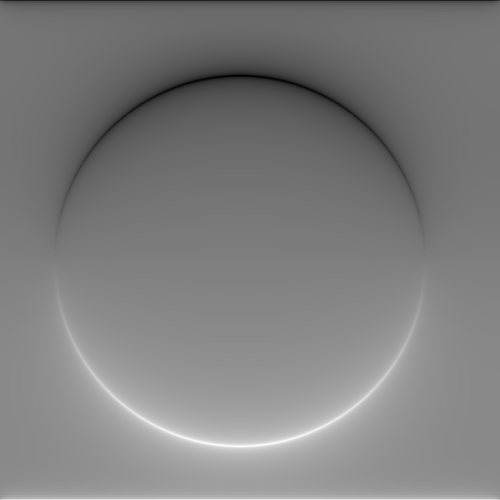
\includegraphics[scale=0.2]{R1disque.png}}
        \subfigure[R2]{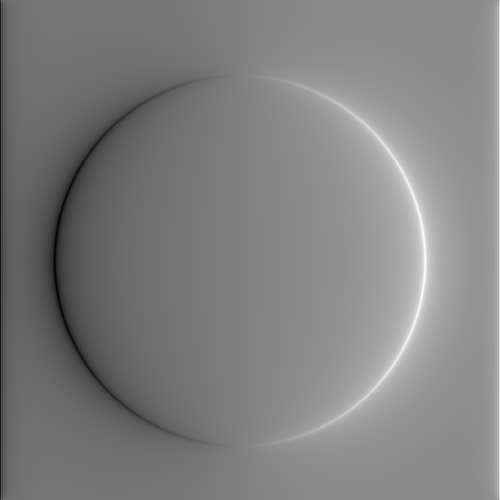
\includegraphics[scale=0.2]{R2disque.png}}
        \subfigure[orientation]{
\includegraphics[scale=0.2]{odisque.png}}
    \end{center}
\end{figure}

\begin{figure}[htbp]
    \begin{center}
        \subfigure[input]{
\includegraphics[scale=0.2]{../images/anneau.png}}
        \subfigure[R1]{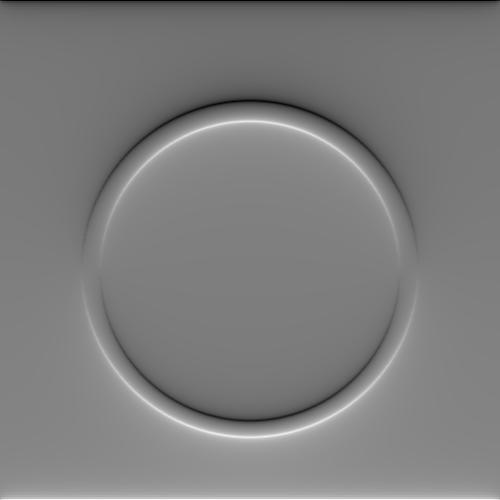
\includegraphics[scale=0.2]{R1anneau.png}}
        \subfigure[R2]{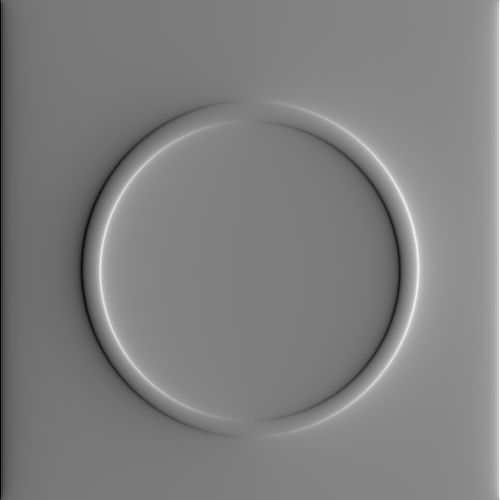
\includegraphics[scale=0.2]{R2anneau.png}}
        \subfigure[orientation]{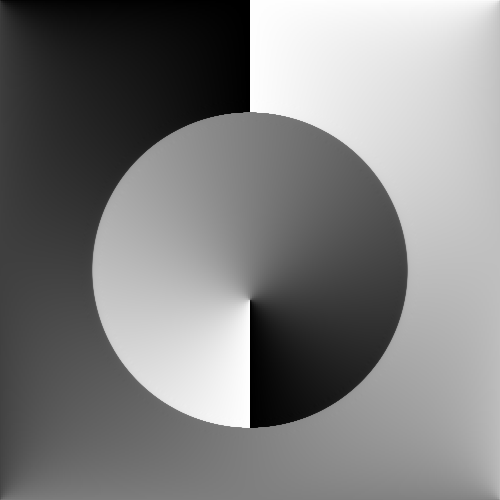
\includegraphics[scale=0.2]{oanneau.png}}
    \end{center}
\end{figure}

\begin{figure}[htbp]
    \begin{center}
        \subfigure[input]{
\includegraphics[scale=0.2]{../images/carre.png}}
        \subfigure[R1]{
\includegraphics[scale=0.2]{R1carre.png}}
        \subfigure[R2]{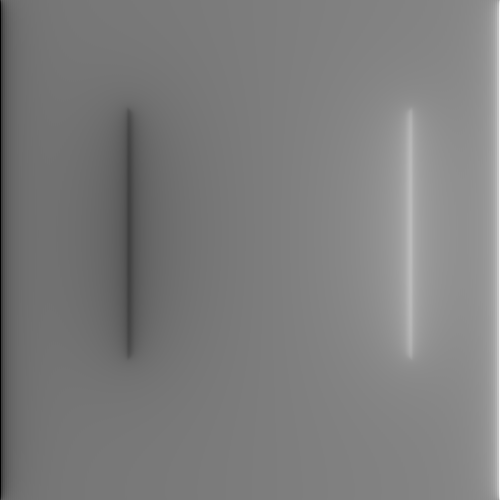
\includegraphics[scale=0.2]{R2carre.png}}
        \subfigure[orientation]{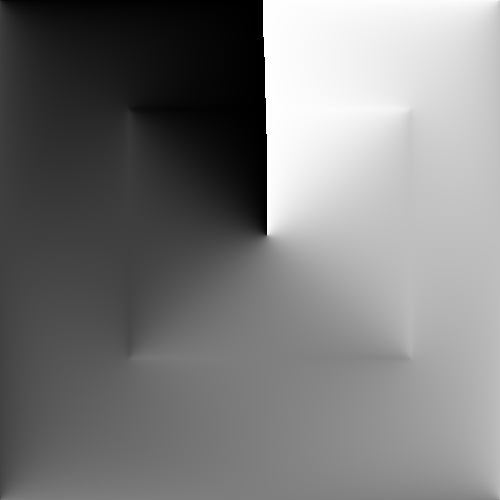
\includegraphics[scale=0.2]{ocarre.png}}
    \end{center}
\end{figure}

\begin{figure}[htbp]
    \begin{center}
        \subfigure[input]{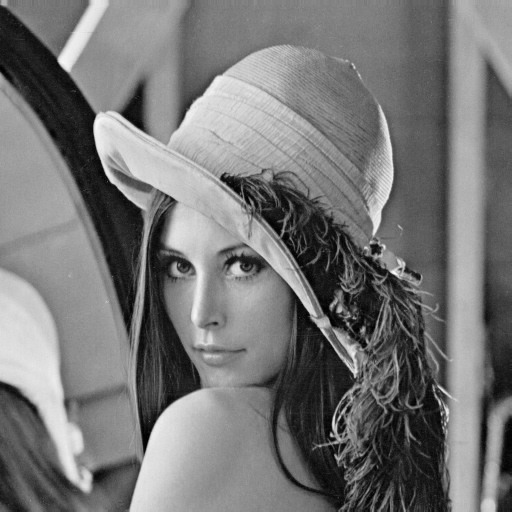
\includegraphics[scale=0.2]{../images/lenna.png}}
        \subfigure[R1]{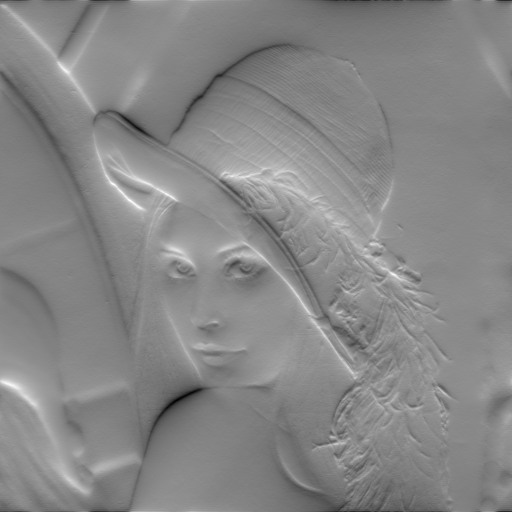
\includegraphics[scale=0.2]{R1lenna.png}}
        \subfigure[R2]{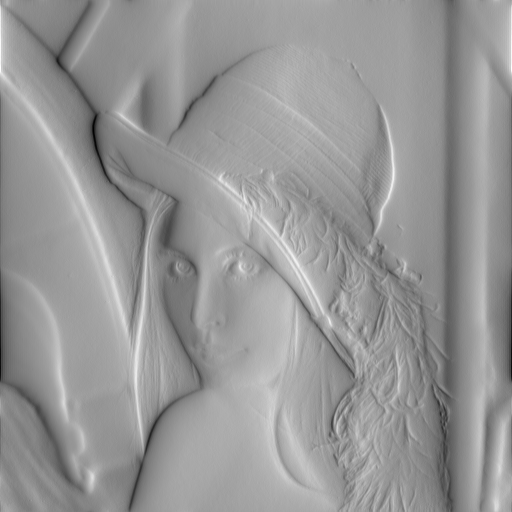
\includegraphics[scale=0.2]{R2lenna.png}}
        \subfigure[orientation]{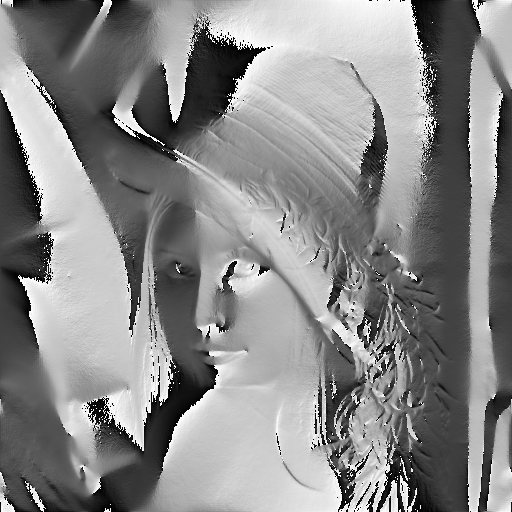
\includegraphics[scale=0.2]{olenna.png}}
    \end{center}
\end{figure}

\begin{figure}[htbp]
    \begin{center}
        \subfigure[input]{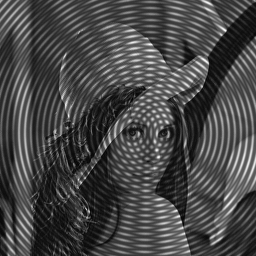
\includegraphics[scale=0.4]{../images/lenna_psyche.png}}
        \subfigure[R1]{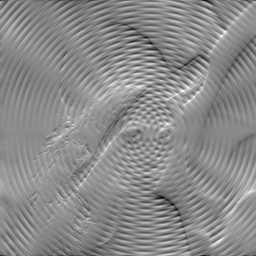
\includegraphics[scale=0.4]{R1lp.png}}
        \subfigure[R2]{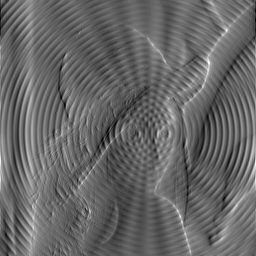
\includegraphics[scale=0.4]{R2lp.png}}
        \subfigure[orientation]{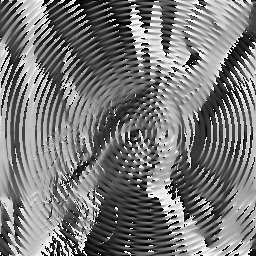
\includegraphics[scale=0.4]{olp.png}}
    \end{center}
\end{figure}

\begin{figure}[htbp]
    \begin{center}
        \subfigure[input]{
\includegraphics[scale=0.1]{../images/cosinus.png}}
        \quad
        \subfigure[R1 th�orique]{
\includegraphics[scale=0.1]{R1_theo_cosinus.png}}
        \quad
        \subfigure[R1 calcul�]{
\includegraphics[scale=0.1]{R1cosinus.png}}
        \quad
        \quad
        \subfigure[R2 th�orique]{
\includegraphics[scale=0.1]{R2_theo_cosinus.png}}
        \quad
        \subfigure[R2 calcul�]{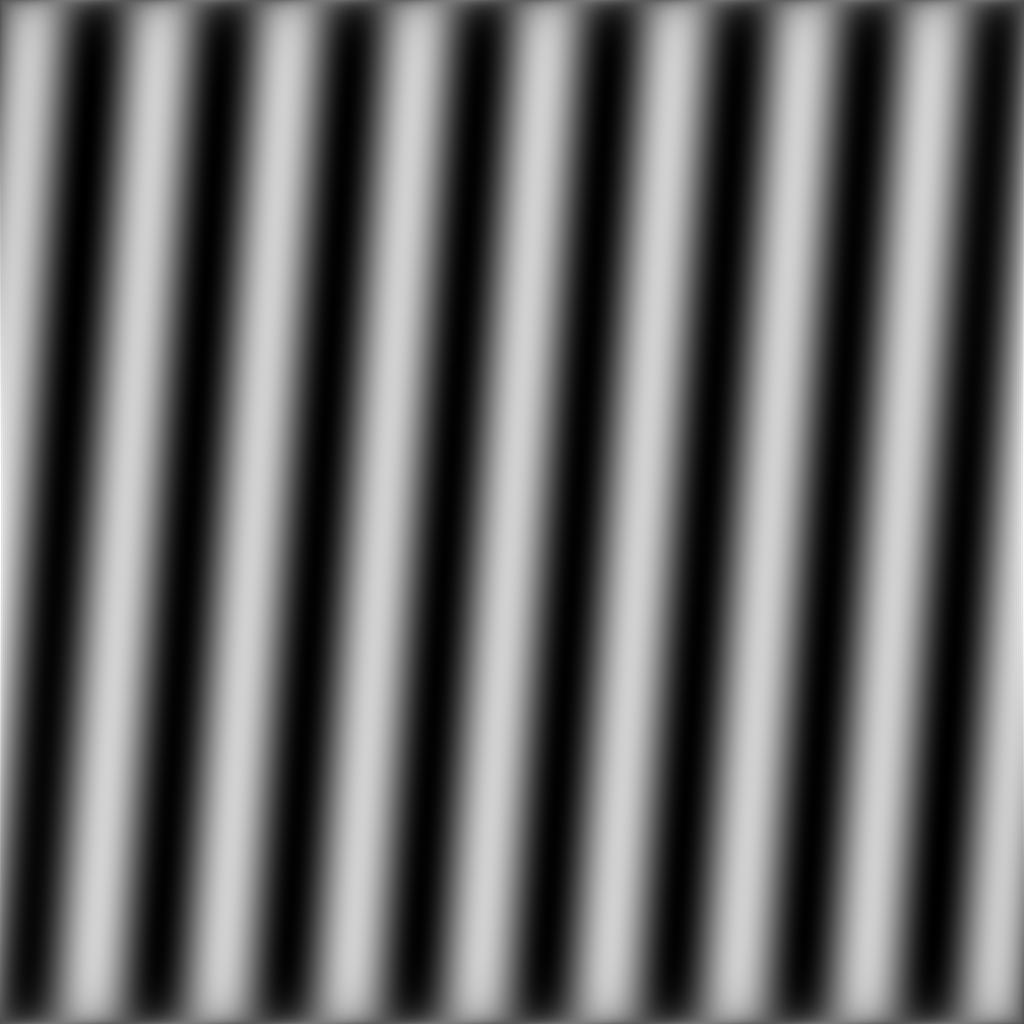
\includegraphics[scale=0.1]{R2cosinus.png}}
        \quad
        \subfigure[orientation]{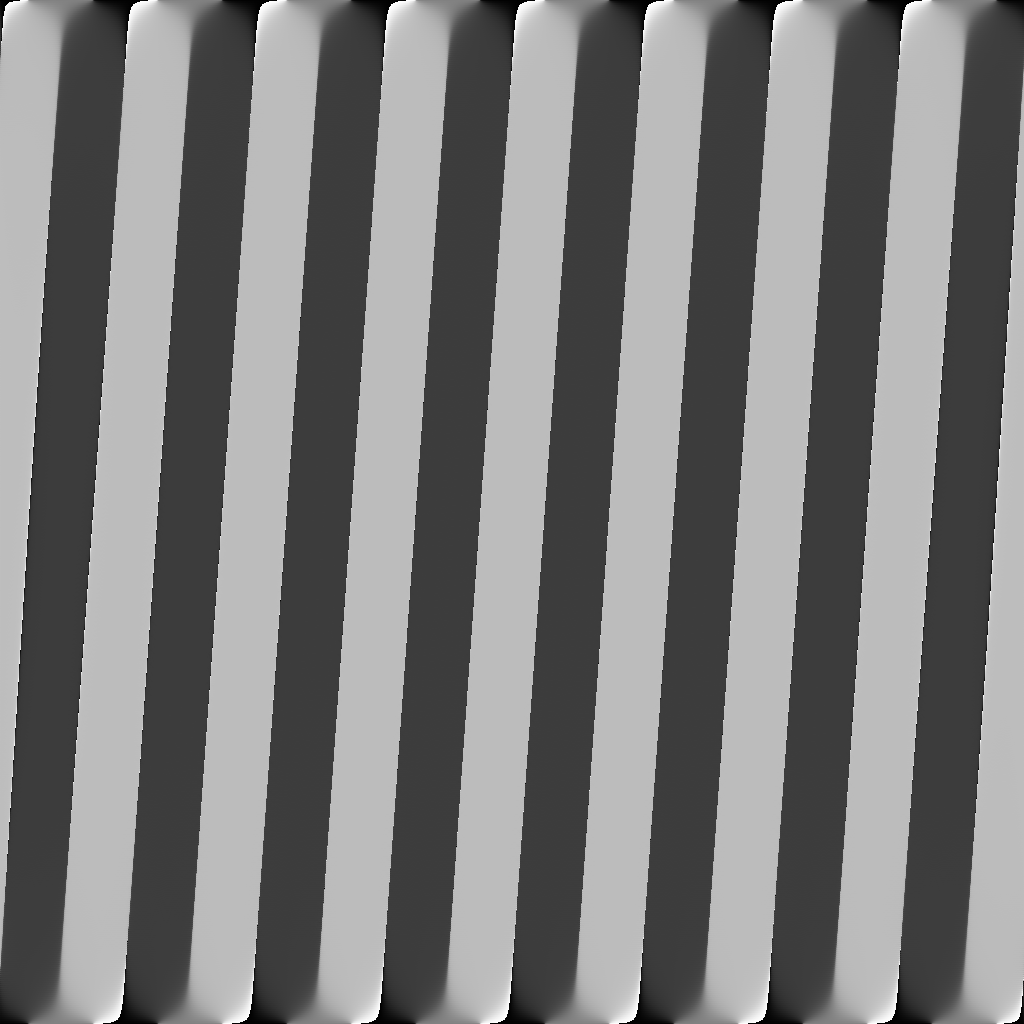
\includegraphics[scale=0.1]{ocosinus.png}}
    \end{center}
\end{figure}

\end{document}
